\section{Exact Values of Small Ramsey Numbers}\label{sec:exact_values}
In this section we compute the exact values of some of the smaller ramsey numbers, using some of the upper bounds which we proved in Section \ref{sec:upper_bound}. The section will be based upon \cite{emogrt}[Chapter 2].
\begin{theorem}\label{thm:small_ramsey_numbers}
	$R(3, 4) = 9, R(3, 5) = 14$ and $R(4, 4) = 18$.
\end{theorem}
\begin{proof}
	by Corollary \ref{cor:upper_bounds_from_ramseys_theorem_even}, we have:
	\begin{equation}\label{eq:R3_4}
		R(3, 4) \leq R(2, 4) + R(3, 3) - 1 = 9
	\end{equation}
	since $R(2, 4) = 4$ and $R(3, 3) = 6$ by Example \ref{exmp:R3_3}. More over by Theorem \ref{thm:ramsey_upper_bound} and Equation \eqref{eq:R3_4} we have:
	\begin{equation}\label{eq:R3_5}
		R(3, 5) \leq R(2, 5) + R(3, 4) \leq 5 + 9 = 14
	\end{equation}
	If we can construct a $2$-edge coloring $\chi: E(K^{*}_{13}) \to \left\{red, blue\right\}$ on $K^{*}_{13}$ with no $red$-clique of order $3$ and no $blue$ clique of order $5$, then we may conclude that $R(3, 5) = 14$ and hence $R(3, 4) = 9$ by Equations \eqref{eq:R3_4} and \eqref{eq:R3_5}. It is in fact the case that we may construct such a $2$-edge coloring $\chi$ on $K^{*}_{13}$ one example of such a coloring is:
	\begin{equation*}
		\chi(\{i, j\}) = \begin{cases}
			red  & \text{ if } [i - j]_{13} \in \left\{1, 5, 8, 12\right\} \\
			blue & \text{ otherwise }
		\end{cases}
	\end{equation*}
	Please note that $\chi$ is well defined since $-1 \equiv 12 \mod 13$ and $-5 \equiv 8 \mod 13$ and hence $[i - j]_{13} \in \left\{1, 5, 8, 12\right\}$ if and only if $[j - i]_{13} \in \left\{1, 5, 8, 12\right\}$. The fact that $\chi$ admits no $red$-monochromatic cliques of order $3$ and no $blue$-monochromatic cliques of order $5$ is checked via the code in Appendix \ref{app:ramsey_code}.
	Additionally since $R(3, 4) = 14$ we have $R(4, 4) \leq R(3, 4) + R(4, 3) = 18$, once again by Theorem \ref{thm:ramsey_upper_bound}, using this inequality we can show that $R(4, 4) = 18$ by constructing a $2$-edge coloring $\gamma: E(K^{*}_{17}) \to \left\{red, blue\right\}$ which admits no $red$ or $blue$ monochromatic cliques of order $4$. One such $2$-edge coloring is given below:
	\begin{equation*}
		\gamma(\left\{i, j\right\}) = \begin{cases}
			red  & \text{ if } [i -  j]_{17} \in \left\{1, 2, 4, 8, 9, 13, 15, 16\right\} \\
			blue & otherwise
		\end{cases}
	\end{equation*}
	again please note that $\gamma$ is well defined, just like $\chi$, by an identical argument. Again the fact that $\gamma$ admits no $red$ or $blue$ monochromatic cliques of order $5$ is checked via the code in Appendix \ref{app:ramsey_code}.
\end{proof}

For the sake of illustration $K^{*}_{13}$ equiped with the $2$-edge coloring $\chi$ and $K^{*}_{17}$ equiped with the $2$-edge coloring $\gamma$, both from the proof of Theorem \ref{thm:small_ramsey_numbers} is illustated below in Figures \ref{fig:small_ramsey_graphs}
\begin{figure}[H]
	\begin{subfigure}[c]{0.4\textwidth}
		\centering
		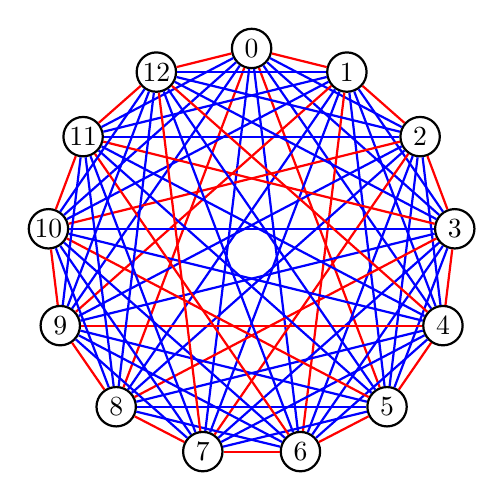
\begin{tikzpicture}
			\tikzset{punkt/.style={circle, thick, draw=black, minimum width=0.5cm,inner sep=0.2}}

			\node[punkt] at (0.0, 2.6) (a) {$0$};
			\node[punkt] at (1.21, 2.3) (b) {$1$};
			\node[punkt] at (2.14, 1.48) (c) {$2$};
			\node[punkt] at (2.58, 0.31) (d) {$3$};
			\node[punkt] at (2.43, -0.92) (e) {$4$};
			\node[punkt] at (1.72, -1.95) (f) {$5$};
			\node[punkt] at (0.62, -2.52) (g) {$6$};
			\node[punkt] at (-0.62, -2.52) (h) {$7$};
			\node[punkt] at (-1.72, -1.95) (i) {$8$};
			\node[punkt] at (-2.43, -0.92) (j) {$9$};
			\node[punkt] at (-2.58, 0.31) (k) {$10$};
			\node[punkt] at (-2.14, 1.48) (l) {$11$};
			\node[punkt] at (-1.21, 2.3) (m) {$12$};
			\draw [thick, draw=red] (a) -- (b);
			\draw [thick, draw=blue] (a) -- (c);
			\draw [thick, draw=blue] (a) -- (d);
			\draw [thick, draw=blue] (a) -- (e);
			\draw [thick, draw=red] (a) -- (f);
			\draw [thick, draw=blue] (a) -- (g);
			\draw [thick, draw=blue] (a) -- (h);
			\draw [thick, draw=red] (a) -- (i);
			\draw [thick, draw=blue] (a) -- (j);
			\draw [thick, draw=blue] (a) -- (k);
			\draw [thick, draw=blue] (a) -- (l);
			\draw [thick, draw=red] (a) -- (m);
			\draw [thick, draw=red] (b) -- (c);
			\draw [thick, draw=blue] (b) -- (d);
			\draw [thick, draw=blue] (b) -- (e);
			\draw [thick, draw=blue] (b) -- (f);
			\draw [thick, draw=red] (b) -- (g);
			\draw [thick, draw=blue] (b) -- (h);
			\draw [thick, draw=blue] (b) -- (i);
			\draw [thick, draw=red] (b) -- (j);
			\draw [thick, draw=blue] (b) -- (k);
			\draw [thick, draw=blue] (b) -- (l);
			\draw [thick, draw=blue] (b) -- (m);
			\draw [thick, draw=red] (c) -- (d);
			\draw [thick, draw=blue] (c) -- (e);
			\draw [thick, draw=blue] (c) -- (f);
			\draw [thick, draw=blue] (c) -- (g);
			\draw [thick, draw=red] (c) -- (h);
			\draw [thick, draw=blue] (c) -- (i);
			\draw [thick, draw=blue] (c) -- (j);
			\draw [thick, draw=red] (c) -- (k);
			\draw [thick, draw=blue] (c) -- (l);
			\draw [thick, draw=blue] (c) -- (m);
			\draw [thick, draw=red] (d) -- (e);
			\draw [thick, draw=blue] (d) -- (f);
			\draw [thick, draw=blue] (d) -- (g);
			\draw [thick, draw=blue] (d) -- (h);
			\draw [thick, draw=red] (d) -- (i);
			\draw [thick, draw=blue] (d) -- (j);
			\draw [thick, draw=blue] (d) -- (k);
			\draw [thick, draw=red] (d) -- (l);
			\draw [thick, draw=blue] (d) -- (m);
			\draw [thick, draw=red] (e) -- (f);
			\draw [thick, draw=blue] (e) -- (g);
			\draw [thick, draw=blue] (e) -- (h);
			\draw [thick, draw=blue] (e) -- (i);
			\draw [thick, draw=red] (e) -- (j);
			\draw [thick, draw=blue] (e) -- (k);
			\draw [thick, draw=blue] (e) -- (l);
			\draw [thick, draw=red] (e) -- (m);
			\draw [thick, draw=red] (f) -- (g);
			\draw [thick, draw=blue] (f) -- (h);
			\draw [thick, draw=blue] (f) -- (i);
			\draw [thick, draw=blue] (f) -- (j);
			\draw [thick, draw=red] (f) -- (k);
			\draw [thick, draw=blue] (f) -- (l);
			\draw [thick, draw=blue] (f) -- (m);
			\draw [thick, draw=red] (g) -- (h);
			\draw [thick, draw=blue] (g) -- (i);
			\draw [thick, draw=blue] (g) -- (j);
			\draw [thick, draw=blue] (g) -- (k);
			\draw [thick, draw=red] (g) -- (l);
			\draw [thick, draw=blue] (g) -- (m);
			\draw [thick, draw=red] (h) -- (i);
			\draw [thick, draw=blue] (h) -- (j);
			\draw [thick, draw=blue] (h) -- (k);
			\draw [thick, draw=blue] (h) -- (l);
			\draw [thick, draw=red] (h) -- (m);
			\draw [thick, draw=red] (i) -- (j);
			\draw [thick, draw=blue] (i) -- (k);
			\draw [thick, draw=blue] (i) -- (l);
			\draw [thick, draw=blue] (i) -- (m);
			\draw [thick, draw=red] (j) -- (k);
			\draw [thick, draw=blue] (j) -- (l);
			\draw [thick, draw=blue] (j) -- (m);
			\draw [thick, draw=red] (k) -- (l);
			\draw [thick, draw=blue] (k) -- (m);
			\draw [thick, draw=red] (l) -- (m);
		\end{tikzpicture}
		\caption{The $2$-edge coloring $\chi$ on $K^{*}_{13}$}
	\end{subfigure}
	\begin{subfigure}[c]{0.6\textwidth}
		\centering
		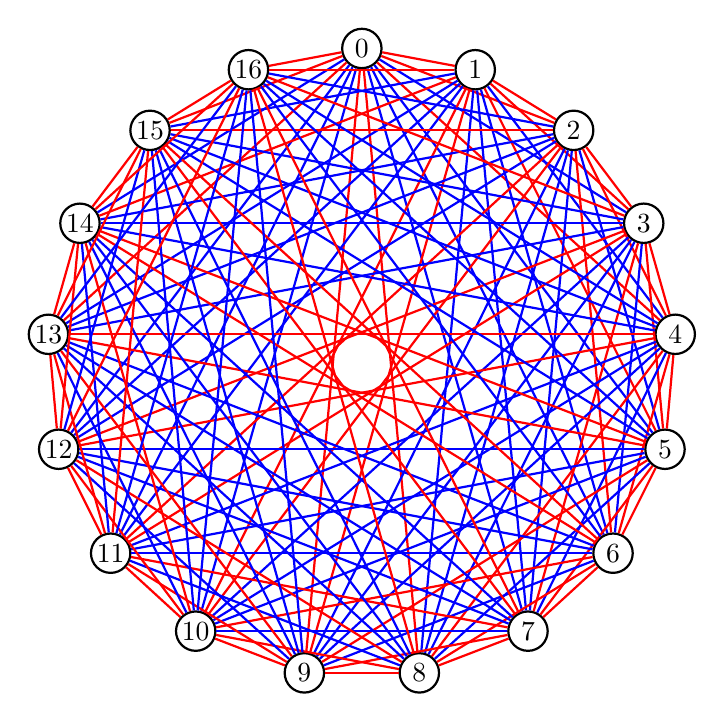
\begin{tikzpicture}
			\tikzset{punkt/.style={circle, thick, draw=black, minimum width=0.5cm,inner sep=0.2}}
			\node[punkt] at (0.0, 4.0) (a) {$0$};
			\node[punkt] at (1.44, 3.73) (b) {$1$};
			\node[punkt] at (2.69, 2.96) (c) {$2$};
			\node[punkt] at (3.58, 1.78) (d) {$3$};
			\node[punkt] at (3.98, 0.37) (e) {$4$};
			\node[punkt] at (3.85, -1.09) (f) {$5$};
			\node[punkt] at (3.19, -2.41) (g) {$6$};
			\node[punkt] at (2.11, -3.4) (h) {$7$};
			\node[punkt] at (0.73, -3.93) (i) {$8$};
			\node[punkt] at (-0.73, -3.93) (j) {$9$};
			\node[punkt] at (-2.11, -3.4) (k) {$10$};
			\node[punkt] at (-3.19, -2.41) (l) {$11$};
			\node[punkt] at (-3.85, -1.09) (m) {$12$};
			\node[punkt] at (-3.98, 0.37) (n) {$13$};
			\node[punkt] at (-3.58, 1.78) (o) {$14$};
			\node[punkt] at (-2.69, 2.96) (p) {$15$};
			\node[punkt] at (-1.44, 3.73) (q) {$16$};
			\draw [thick, draw=red] (a) -- (b);
			\draw [thick, draw=red] (a) -- (c);
			\draw [thick, draw=blue] (a) -- (d);
			\draw [thick, draw=red] (a) -- (e);
			\draw [thick, draw=blue] (a) -- (f);
			\draw [thick, draw=blue] (a) -- (g);
			\draw [thick, draw=blue] (a) -- (h);
			\draw [thick, draw=red] (a) -- (i);
			\draw [thick, draw=red] (a) -- (j);
			\draw [thick, draw=blue] (a) -- (k);
			\draw [thick, draw=blue] (a) -- (l);
			\draw [thick, draw=blue] (a) -- (m);
			\draw [thick, draw=red] (a) -- (n);
			\draw [thick, draw=blue] (a) -- (o);
			\draw [thick, draw=red] (a) -- (p);
			\draw [thick, draw=red] (a) -- (q);
			\draw [thick, draw=red] (b) -- (c);
			\draw [thick, draw=red] (b) -- (d);
			\draw [thick, draw=blue] (b) -- (e);
			\draw [thick, draw=red] (b) -- (f);
			\draw [thick, draw=blue] (b) -- (g);
			\draw [thick, draw=blue] (b) -- (h);
			\draw [thick, draw=blue] (b) -- (i);
			\draw [thick, draw=red] (b) -- (j);
			\draw [thick, draw=red] (b) -- (k);
			\draw [thick, draw=blue] (b) -- (l);
			\draw [thick, draw=blue] (b) -- (m);
			\draw [thick, draw=blue] (b) -- (n);
			\draw [thick, draw=red] (b) -- (o);
			\draw [thick, draw=blue] (b) -- (p);
			\draw [thick, draw=red] (b) -- (q);
			\draw [thick, draw=red] (c) -- (d);
			\draw [thick, draw=red] (c) -- (e);
			\draw [thick, draw=blue] (c) -- (f);
			\draw [thick, draw=red] (c) -- (g);
			\draw [thick, draw=blue] (c) -- (h);
			\draw [thick, draw=blue] (c) -- (i);
			\draw [thick, draw=blue] (c) -- (j);
			\draw [thick, draw=red] (c) -- (k);
			\draw [thick, draw=red] (c) -- (l);
			\draw [thick, draw=blue] (c) -- (m);
			\draw [thick, draw=blue] (c) -- (n);
			\draw [thick, draw=blue] (c) -- (o);
			\draw [thick, draw=red] (c) -- (p);
			\draw [thick, draw=blue] (c) -- (q);
			\draw [thick, draw=red] (d) -- (e);
			\draw [thick, draw=red] (d) -- (f);
			\draw [thick, draw=blue] (d) -- (g);
			\draw [thick, draw=red] (d) -- (h);
			\draw [thick, draw=blue] (d) -- (i);
			\draw [thick, draw=blue] (d) -- (j);
			\draw [thick, draw=blue] (d) -- (k);
			\draw [thick, draw=red] (d) -- (l);
			\draw [thick, draw=red] (d) -- (m);
			\draw [thick, draw=blue] (d) -- (n);
			\draw [thick, draw=blue] (d) -- (o);
			\draw [thick, draw=blue] (d) -- (p);
			\draw [thick, draw=red] (d) -- (q);
			\draw [thick, draw=red] (e) -- (f);
			\draw [thick, draw=red] (e) -- (g);
			\draw [thick, draw=blue] (e) -- (h);
			\draw [thick, draw=red] (e) -- (i);
			\draw [thick, draw=blue] (e) -- (j);
			\draw [thick, draw=blue] (e) -- (k);
			\draw [thick, draw=blue] (e) -- (l);
			\draw [thick, draw=red] (e) -- (m);
			\draw [thick, draw=red] (e) -- (n);
			\draw [thick, draw=blue] (e) -- (o);
			\draw [thick, draw=blue] (e) -- (p);
			\draw [thick, draw=blue] (e) -- (q);
			\draw [thick, draw=red] (f) -- (g);
			\draw [thick, draw=red] (f) -- (h);
			\draw [thick, draw=blue] (f) -- (i);
			\draw [thick, draw=red] (f) -- (j);
			\draw [thick, draw=blue] (f) -- (k);
			\draw [thick, draw=blue] (f) -- (l);
			\draw [thick, draw=blue] (f) -- (m);
			\draw [thick, draw=red] (f) -- (n);
			\draw [thick, draw=red] (f) -- (o);
			\draw [thick, draw=blue] (f) -- (p);
			\draw [thick, draw=blue] (f) -- (q);
			\draw [thick, draw=red] (g) -- (h);
			\draw [thick, draw=red] (g) -- (i);
			\draw [thick, draw=blue] (g) -- (j);
			\draw [thick, draw=red] (g) -- (k);
			\draw [thick, draw=blue] (g) -- (l);
			\draw [thick, draw=blue] (g) -- (m);
			\draw [thick, draw=blue] (g) -- (n);
			\draw [thick, draw=red] (g) -- (o);
			\draw [thick, draw=red] (g) -- (p);
			\draw [thick, draw=blue] (g) -- (q);
			\draw [thick, draw=red] (h) -- (i);
			\draw [thick, draw=red] (h) -- (j);
			\draw [thick, draw=blue] (h) -- (k);
			\draw [thick, draw=red] (h) -- (l);
			\draw [thick, draw=blue] (h) -- (m);
			\draw [thick, draw=blue] (h) -- (n);
			\draw [thick, draw=blue] (h) -- (o);
			\draw [thick, draw=red] (h) -- (p);
			\draw [thick, draw=red] (h) -- (q);
			\draw [thick, draw=red] (i) -- (j);
			\draw [thick, draw=red] (i) -- (k);
			\draw [thick, draw=blue] (i) -- (l);
			\draw [thick, draw=red] (i) -- (m);
			\draw [thick, draw=blue] (i) -- (n);
			\draw [thick, draw=blue] (i) -- (o);
			\draw [thick, draw=blue] (i) -- (p);
			\draw [thick, draw=red] (i) -- (q);
			\draw [thick, draw=red] (j) -- (k);
			\draw [thick, draw=red] (j) -- (l);
			\draw [thick, draw=blue] (j) -- (m);
			\draw [thick, draw=red] (j) -- (n);
			\draw [thick, draw=blue] (j) -- (o);
			\draw [thick, draw=blue] (j) -- (p);
			\draw [thick, draw=blue] (j) -- (q);
			\draw [thick, draw=red] (k) -- (l);
			\draw [thick, draw=red] (k) -- (m);
			\draw [thick, draw=blue] (k) -- (n);
			\draw [thick, draw=red] (k) -- (o);
			\draw [thick, draw=blue] (k) -- (p);
			\draw [thick, draw=blue] (k) -- (q);
			\draw [thick, draw=red] (l) -- (m);
			\draw [thick, draw=red] (l) -- (n);
			\draw [thick, draw=blue] (l) -- (o);
			\draw [thick, draw=red] (l) -- (p);
			\draw [thick, draw=blue] (l) -- (q);
			\draw [thick, draw=red] (m) -- (n);
			\draw [thick, draw=red] (m) -- (o);
			\draw [thick, draw=blue] (m) -- (p);
			\draw [thick, draw=red] (m) -- (q);
			\draw [thick, draw=red] (n) -- (o);
			\draw [thick, draw=red] (n) -- (p);
			\draw [thick, draw=blue] (n) -- (q);
			\draw [thick, draw=red] (o) -- (p);
			\draw [thick, draw=red] (o) -- (q);
			\draw [thick, draw=red] (p) -- (q);
		\end{tikzpicture}
		\caption{The $2$-edge coloring $\gamma$ on $K^{*}_{17}$}
	\end{subfigure}
	\caption{The two 2-edge colorings described in the proof of Theorem \ref{thm:small_ramsey_numbers} illustrated.}
	\label{fig:small_ramsey_graphs}
\end{figure}


Before moving on we will need one additional concept, introduced in the following definition:
\begin{definition}\label{def:set_sum_free}
	Let $(G, +)$ be an abelian group, then the subset $S \subseteq G$ is called \textit{sum-free} if the equation $x + y = z$ has no solution in $S$.
\end{definition}

Some parts of the proof of the following Theorem is inspired by \cite{graph_theory}[Exercise 12.3.4]
\begin{theorem}\label{thm:R3_3_3}
	We have $R(3, 3, 3) = 17$.
\end{theorem}
\begin{proof}
	We start by showing that any $3$-edge coloring $\chi: E(K_{17}) \to \left\{red, blue, green\right\}$ admits a monochromatic clique of order $3$. Let $v \in V(K_{17})$, by the generalized pigeonhole principle (Theorem \ref{thm:gpp}), there exists a color $c \in \left\{red, blue, green\right\}$ such that $\abs{\mathcal{N}_{\chi}(v; c)} \geq 6$. Assume without loss of generalization that $c = red$, then we may assume that $\chi\left(E(K_{17} \vert_{\mathcal{N}_{\chi}(v; c)})\right) = \left\{blue, green\right\}$, otherwise we would have a $red$-monochromatic clique of order $3$. However since $R(3, 3) = 6$, this means that $\chi$ admits either a $blue$ or $green$ monochromatic clique of order $3$.

	Next we will show that $R(3, 3, 3) > 16$, we will do this by constructing a $3$-edge coloring $\gamma$ on the complete graph $K$ with vertex set $\mathbb{Z}_2[X] / \gen{X^4 + X + 1}$\footnote{Which is of course isomorphic to $\mathbb{F}_{16}$, however it will be move convinient for us to work from this polynomial view.}. We will construct $3$ cosets $S_{red}, S_{blue}, S_{green}$ which partition $\mathbb{Z}_2[X] / \gen{X^4 + X + 1}$, and assign a color to the edge $\left\{v, u\right\}$ according to which coset $v + u$ belongs to. To start let:
	\begin{equation*}
		S_{red} := \left\{X^3, X^2 + X^{3}, X + X^{3}, 1 + X + X^2 + X^3 , 1\right\}
	\end{equation*}
	Note that $S_{red}$ is a subgroup of the multiplicative group $(\mathbb{Z}_2[X] / \gen{X^4 + X + 1})^{*}$, additionally we note that $S_{red}$ is sum-free, which is easy albeit cumbersome to check. Similarly we let $A_{blue} := X S_{red}$ and $S_{green} := X^2 S_{red}$, these cosets must also be sum-free since $a + b = c$ with $a, b, c \in S_{blue}$ or $a, b, c \in S_{green}$ would imply:
	\begin{equation*}
		Xa' + Xb' = Xc' \implies a' + b' = c' \text{ with } a', b', c' \in S_{red}
	\end{equation*}
	or
	\begin{equation*}
		X^{2}a' + X^{2}b' = X^{2}c' \implies a' + b' = c' \text{ with } a', b', c' \in S_{red}
	\end{equation*}
	respectively, since $\mathbb{Z}_2[X] / \gen{X^4 + X + 1}$ is a finite field and hence a domain. Define $\gamma(\left\{v, u\right\}) = c$ if and only if $v + u \in S_{c}$, additionally we note that $\gamma$ is well defined as $v \neq u$ and $\Char(\mathbb{Z}_2[X] / \gen{X^4 + X + 1}) = 2$. Assume for the sake of contradiction that $\gamma$ admits a $c$-monochromatic clique of order $3$, that is there exists $u, v, w \in V(K) = \mathbb{Z}_2[X] / \gen{X^4 + X + 1}$ such that $u + v, u + w, v + w \in S_c$, then $u + w = (u + v) + (v + w)$ contradicting the fact that $S_c$ is sum-free.
\end{proof}

Finally we present a summary of the exact values and bounds for small Ramsey numbers, below in Table \ref{tab:small_values}:
\begin{table}[H]
	\centering
	\begin{tabular} {||c|c|c|c|c||}
		\hline
		$\ell_1 \setminus \ell_{2}$ & $2$ & $3$  & $4$                     & $5$                      \\
		\hline
		$2$                         & $2$ & $3$  & $4$                     & $5$                      \\
		\hline
		$3$                         & $3$ & $6$  & $9$                     & $14$                     \\
		\hline
		$4$                         & $4$ & $9$  & $18$                    & $\leq31$, $\mathbf{25}$  \\
		\hline
		$5$                         & $5$ & $14$ & $\leq31$, $\mathbf{25}$ & $\leq62$, \textbf{43-48} \\
		\hline
	\end{tabular}
	\caption{Some exact values and bounds for small Ramsey numbers. The bold entries are exact values or best known bounds, if the exact value is unknown, which we have not covered in this project. The bold values are sourced from \cite{small_values}.}
	\label{tab:small_values}
\end{table}
